\newpage
\section{Процесс загрузки приложений Windows}

\subsection{Выполнение ЕХЕ-модуля}

При запуске ЕХЕ-файла (сокр. англ. executable — исполнимый) загрузчик операционной системы создает для его процесса виртуальное адресное пространство и проецирует на него исполняемый модуль. Далее загрузчик анализирует раздел импорта и пытается спроецировать все необходимые DLL на адресное пространство процесса.

Поскольку в разделе импорта указано только имя DLL (без пути), загрузчику приходится самому искать ее на дисковых устройствах в компьютере пользователя. Поиск DLL осуществляется в следующей последовательности.

\begin{itemize}
\item Каталог, содержащий ЕХЕ-файл.
\item Текущий каталог процесса.
\item Системный каталог Windows
\item Основной каталог Windows
\item Каталоги, указанные в переменной окружения PATH.
\end{itemize}

Проецируя DLL-модули на адресное пространство, загрузчик проверяет в каждом из них раздел импорта. Если у DLL есть раздел импорта (что обычно бывает), загрузчик проецирует следующий DLL-модуль. При этом загрузчик ведет учет загружаемых DLL и проецирует их только один раз, даже если загрузки этих DLL требуют и другие модули.

Если найти файл DLL не удается, загрузчик выводит сообщение об ошибке.

Найдя и спроецировав на адресное пространство процесса все необходимые DLL-модули, загрузчик настраивает ссылки на импортируемые идентификаторы. Для этого он вновь просматривает разделы импорта в каждом модуле, проверяя наличие указанного идентификатора в соответствующей DLL.

Если идентификатор не найден, то это заканчивается выводом сообщения об ошибке, если же идентификатор найден, загрузчик отыскивает его RVA и прибавляет к виртуальному адресу, по которому данная DLL размещена в адресном пространстве процесса, а затем сохраняет полученный виртуальный адрес в разделе импорта EXE-модуля. И с этого момента ссылка в коде на импортируемый идентификатор приводит к выборке его адреса из раздела импорта вызывающего модуля, открывая таким образом доступ к импортируемой переменной, функции или функции-члену C++ класса. После этого динамические связи установлены, первичный поток процесса начал выполняться, и приложение начинает работать\cite{Cit4}.

Загрузка всех DLL и настройка ссылок занимает какое-то время, но, поскольку такие операции выполняются лишь при запуске процесса, на производительности приложения это не сказывается Тем не менее, для многих программ подобная задержка при инициализации неприемлема. Чтобы сократить время загрузки приложения, можно модифицировать базовые адреса EXE- и DLL-модулей и провести их (модулей) связывание.

\subsection{Динамически подключаемые библиотеки}

Динамические библиотеки (dynamic-link libraries, DLL) -- краеугольный камень операционной системы Windows, начиная с самой первой ec версии. В DLL содержатся все функции Windows API. Три самые важные DLL:
\begin{itemize}
\item Kernel32.dll -- управление памятью, процессами и потоками
\item User32.dll -- поддержка пользовательского интерфейса, в том числе функции, связанные с созданием окон и передачей сообщений
\item GDI32.dll -- графика и вывод текста.
\end{itemize}

В Windows есть и другие DLL, функции которых предназначены для более специализированных задач. Например, в AdvAPI32.dll содержатся функции для защиты объектов, работы с реестром и регистрации событий, в ComDlg32.dll -- стандартные диалоговые окна (вроде File Open и File Save), a ComCrl32.dll поддерживает стандартные элементы управления.

Вот основные причины, по которым инструмент DLL получил такую популярность:
\begin{itemize}
\item \textbf{Расширение функциональности приложения}. DLL можно загружать в адресное пространство процесса динамически, что позволяет приложению, определив, какие действия от него требуются, подгружать нужный код. Поэтому одна компания, создав какое-то приложение, может предусмотреть расширение его функциональности за счет DLL от других компаний.
\item \textbf{Возможность использования разных языков программирования}. У разработчика есть выбор, на каком языке писать ту или иную часть приложения. Пользовательский интерфейс приложения можно создавать на Microsoft Visual Basic, а прикладную реализовать на С++. Программа на Visual Basic может загружать DLL, написанные на С++, Коболе, Фортране и др.
\item \textbf{Более простое управление проектом}. Если в процессе разработки программного продукта отдельные его модули создаются разными группами, то при использовании DLL таким проектом управлять гораздо проще. Однако конечная версия приложения должна включать как можно меньше файлов.
\item \textbf{Экономия памяти}. Если одну и ту же DLL использует несколько приложений, в оперативной памяти может храниться только один ее экземпляр, доступный этим приложениям. Пример -- DLL-версия библиотеки С/С++. Эту библиотеку используют многие приложения. Если всех их скомпоновать со статически подключаемой версией этой библиотеки, то код таких функций, как sprintf, strcpy, malloc и др., будет многократно дублироваться в памяти. Но если они компонуются с DLL-версией библиотеки С/С++, в памяти будет присутствовать лишь одна копия кода этих функций, что позволит гораздо эффективнее использовать оперативную память.
\item \textbf{Разделение ресурсов}. DLL могут содержать такие ресурсы, как шаблоны диалоговых окон, строки, значки и битовые карты (растровые изображения). Эти ресурсы доступны любым программам.
\item \textbf{Упрощение локализации}. DLL нередко применяются для локализации приложений. Например, приложение, содержащее только код без всяких компонентов пользовательского интерфейса, может загружать DLL с компонентами локализованного интерфейса
\item Решение проблем, связанных с \textbf{особенностями различных платформ}. В разных версиях Windows содержатся разные наборы функций. Зачастую разработчикам нужны новые функции, существующие в той версии системы, которой они пользуются. Если Windows пользователя не поддерживает эти функции, ему не удастся запустить такое приложение: загрузчик попросту откажется его запускать. Но если эти функции будут находиться в отдельной DLL, можно будет загрузить программу даже в более ранних версиях Windows.
\item \textbf{Реализация специфических возможностей}. Определенная функциональность в Windows доступна только при использовании DLL Например, отдельные виды ловушек (устанавливаемых вызовом SetWindowsHookEx и SetWinEventHook) можно задействовать при том условии, что функция уведомления ловушки размещена в DLL. Кроме того, расширение функциональности оболочки Windows возможно лишь за счет создания СОМ-объектов, существование которых допустимо только в DLL. Это же относится и к загружаемым Web-браузером ActiveX-элементам, позволяющим создавать Web-страницы с более богатой функциональностью.
\end{itemize}

Зачастую создать DLL проще, чем приложение, потому что она является лишь набором автономных функций, пригодных для использования любой программой, причем в DLL обычно нет кода, предназначенного для обработки циклов выборки сообщений или создания окон. DLL представляет собой набор модулей исходного кода, в каждом из которых содержится определенное число функций, вызываемых приложением (исполняемым файлом) или другими DLL. Файлы с исходным кодом компилируются и компонуются так же, как и при создании ЕХЕ-файла. Но, создавая DLL, нужно указывать компоновщику ключ /DLL. Тогда компоновщик записывает в конечный файл информацию, по которой загрузчик операционной системы определяет, что данный файл -- DLL, а не приложение

Чтобы приложение (или другая DLL) могло вызывать функции, содержащиеся в DLL, образ ее файла нужно сначала спроецировать на адресное пространство вызывающего процесса. Это достигается либо за счёт неявного связывания при загрузке, либо за счет явного -- в период выполнения.

Как только DLL спроецирована на адресное пространство вызывающего процесса, ее функции доступны всем потокам этого процесса. Фактически библиотеки при этом теряют почти всю индивидуальность: для потоков код и данные DLL -- просто дополнительные код и данные, оказавшиеся в адресном пространстве процесса. Когда поток вызывает из DLL какую-то функцию, та считывает свои параметры из стека потока и размещает в этом стеке собственные локальные переменные. Кроме того, любые созданные кодом DLL объекты принадлежат вызывающему потоку или процессу -- DLL ничем пе владеет.

Например, если DLL-функция вызывает VirtualAlloc, резервируется регион в адресном пространстве того процесса, которому принадлежит поток, обратившийся к DLL-функции. Если DLL будет выгружена из адресного пространства процесса, зарезервированный регион не освободится, так как система не фиксирует того, что регион зарезервирован DLL-функций. Считается, что он принадлежит процессу и поэтому освободится, только если поток этого процесса вызовет VirtualFree или завершится сам процесс.

\subsection{Реализация резидентного приложения}

Как и в случае с Linux, приложение отображает количество переданной и полученной информации сетевым интерфейсом. Тут интересно, что используемую в процессе функцию мы получаем непосредственно во время работы (стр. 20 - 22, листинг 7).

\lstinputlisting[language=C++, caption={Утилита сбора информации о трафике на сетевых интерфейсах (src/ELF/win/main.cpp)}]
{../../src/ELF/win/main.cpp}

Результат выполнения программы представлен на рисунке 4.

Заполнение таблицы с информацией об интерфейсах (стр. 37, листинг 7) вынесена в отдельную функцию (стр.34, листинг 7). В приложении производится большое количество обращений к различным DLL. Для упрощения дальнейшего анализа вынесем функцию в отдельную динамическую библиотеку (myDllLib) и продолжим анализ.

\begin{figure}[H]
 \centering
 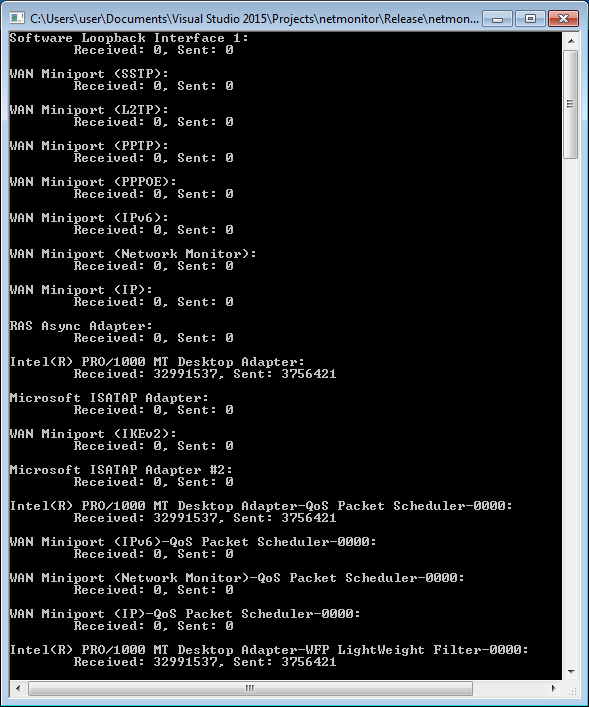
\includegraphics[scale=1]{res/win_004}
 \caption{Исполнение программы в среде Windows}
\end{figure}

\subsection{Анализ исполнения приложения}

Утилита API Monitor может декодировать параметры функций и возвращаемые значения, чтобы представить их в понятном формате, а также отобразить точки обращения разработанной динамической myDllLib.dll
\begin{Verbatim}[frame=single]
	#	Time of Day	Thread	Module	API	Return Value	Error	Duration
	14013	12:11:01.054 PM	1	myDllLib.dll	DecodePointer ( 0xae11ecb8 )	0x004cb8b0		0.0000015
	14014	12:11:01.054 PM	1	myDllLib.dll	DecodePointer ( 0xae11ec98 )	0x004cb8b8		0.0000005
	14015	12:11:01.054 PM	1	myDllLib.dll	EncodePointer ( NULL )	0xaf230e78		0.0000006
	14016	12:11:01.054 PM	1	myDllLib.dll	DecodePointer ( 0xd6ff4bcd )	0x5e77116d		0.0000005
	14017	12:11:01.054 PM	1	myDllLib.dll	EncodePointer ( NULL )	0xaf230e78		0.0000004
				
	#	Time of Day	Thread	Module	API	Return Value	Error	Duration
	14020	12:11:01.054 PM	1	myDllLib.dll	DecodePointer ( 0xae11ecb8 )	0x004cb8b0		0.0000005
	14021	12:11:01.054 PM	1	myDllLib.dll	DecodePointer ( 0xae11ec98 )	0x004cb8b8		0.0000005
	14022	12:11:01.054 PM	1	myDllLib.dll	EncodePointer ( NULL )	0xaf230e78		0.0000004
	14023	12:11:01.054 PM	1	myDllLib.dll	DecodePointer ( 0xd6ff4ef5 )	0x5e771023		0.0000004
	14024	12:11:01.054 PM	1	myDllLib.dll	EncodePointer ( NULL )	0xaf230e78		0.0000005
	14025	12:11:01.054 PM	1	myDllLib.dll	DecodePointer ( 0xae11ecb8 )	0x004cb8b0		0.0000005
	14026	12:11:01.054 PM	1	myDllLib.dll	DecodePointer ( 0xae11ec98 )	0x004cb8b8		0.0000004
\end{Verbatim}

Отладчик OllyDbg позволяет осуществить разбор пользовательского режима (ring 3). При запуске программы, изначальной точкой входа является функция \_tmainCRTStartup. Ниже приведена команда вызова данной функции:
\begin{Verbatim}[frame=single]
	CPU Disasm Address Hex dump      Command                 Comments
	01271BA3  |.      E8 ADF4FFFF CALL 01271055;          [__security_init_cookie
	01271BA8  |.      E8 73FCFFFF CALL __tmainCRTStartup; [__tmainCRTStartup
\end{Verbatim}

Сама функция \_tmainCRTStartup находится по адресу 012F1820:
\begin{Verbatim}[frame=single]
	CPU Disasm
	Address   Hex dump Command  Comments
	012F1820  /$  55  PUSH EBP; INT myDllTest.__tmainCRTStartup(void)	
\end{Verbatim}

Адрес начала подключения динамической библиотеки находится по адресу 012F1820:
\begin{Verbatim}[frame=single]
	CPU Disasm
	Address   Hex dump        Command   Comments
	012F1820  /$  55        PUSH EBP;   INT myDllTest.__tmainCRTStartup(void)
	012F1821  |.  8BEC          MOV EBP,ESP
	012F1823  |.  6A FE         PUSH -2
	012F1825  |.  68 D06E2F01   PUSH OFFSET 012F6ED0
	012F182A  |.  68 7D102F01   PUSH 012F107D
	012F182F  |.  64:A1 0000000 MOV EAX,DWORD PTR FS:[0]
	012F1835  |.  50            PUSH EAX
	012F1836  |.  83C4 E4       ADD ESP,-1C
	012F1839  |.  53            PUSH EBX
	012F183A  |.  56            PUSH ESI
	012F183B  |.  57            PUSH EDI
	012F183C  |.  A1 24802F01   MOV EAX,DWORD PTR DS:[__security_cookie]
	012F1841  |.  3145 F8       XOR DWORD PTR SS:[EBP-8],EAX
	012F1844  |.  33C5          XOR EAX,EBP
	012F1846  |.  50            PUSH EAX
	012F1847  |.  8D45 F0       LEA EAX,[EBP-10]
	012F184A  |.  64:A3 0000000 MOV DWORD PTR FS:[0],EAX
	012F1850  |.  8965 E8       MOV DWORD PTR SS:[EBP-18],ESP
	012F1853  |.  C745 FC 00000 MOV DWORD PTR SS:[EBP-4],0
	012F185A  |.  C745 E4 00000 MOV DWORD PTR SS:[EBP-1C],0
\end{Verbatim}
Адреса точки входа и подключения библиотек не изменились.

Process Monitor является усовершенствованным инструментом отслеживания для Windows, который в режиме реального времени отображает активность файловой системы, реестра, а также процессов и потоков. Проверим адреса подключения динамической библиотеки при помощи утилиты Process Monitor.
\begin{Verbatim}[frame=single]
	Description:	
	Company:	
	Name:	myDllTest.exe
	Version:	
	Path:	C:\Projects\myDllLib\Debug\myDllTest.exe
	Command Line:	myDllTest.exe
	PID:	3380
	Parent PID:	2436
	Session ID:	1
	User:	sba-PC\sba
	Auth ID:	00000000:0001b9ac
	Architecture:	32-bit
	Virtualized:	False
	Integrity:	Обязательная метка\Средний обязательный уровень
	Started:	22.03.2016 2:02:47
	Ended:	22.03.2016 2:04:46
	Modules:
	myDllTest.exe	0x250000	0x1c000	C:\Projects\myDllLib\Debug\myDllTest.exe
	22.03.2016 0:45:34
	MSVCR120D.dll	0x72e10000	0x1bf000	C:\Windows\SysWOW64\MSVCR120D.dll
	Microsoft Corporation	12.00.21005.1 built by: REL	05.10.2013 5:43:49
	myDllLib.dll	0x73be0000	0x1b000	C:\Projects\myDllLib\Debug\myDllLib.dll
	22.03.2016 0:45:33
	wow64win.dll	0x74b40000	0x5c000	C:\Windows\SYSTEM32\wow64win.dll
	Microsoft Corporation	6.1.7601.19018 (win7sp1_gdr.150928-1507)	29.09.2015 6:12:11
	wow64.dll	0x74ba0000	0x3f000	C:\Windows\SYSTEM32\wow64.dll
	Microsoft Corporation	6.1.7601.19018
	(win7sp1_gdr.150928-1507)	29.09.2015 6:12:08
	wow64cpu.dll	0x74c10000	0x8000	C:\Windows\SYSTEM32\wow64cpu.dll	Microsoft
	Corporation	6.1.7601.19018 (win7sp1_gdr.150928-1507)
	29.09.2015 6:12:09
	KERNELBASE.dll	0x75220000	0x47000	C:\Windows\syswow64\KERNELBASE.dll	Microsoft
	Corporation	6.1.7601.18015 (win7sp1_gdr.121129-1432)
	29.09.2015 6:00:36
	kernel32.dll	0x75350000	0x110000	C:\Windows\syswow64\kernel32.dll	Microsoft
	Corporation	6.1.7601.18015 (win7sp1_gdr.121129-1432)
	29.09.2015 6:00:35
	ntdll.dll	0x77100000	0x1a9000	C:\Windows\SYSTEM32\ntdll.dll
	Microsoft Corporation	6.1.7600.16385
	(win7_rtm.090713-1255)	29.09.2015 6:07:47
	ntdll.dll	0x772e0000	0x180000	C:\Windows\SysWOW64\ntdll.dll
	Microsoft Corporation	6.1.7600.16385
	(win7_rtm.090713-1255)	29.09.2015 5:57:52
\end{Verbatim}
Как видно из вывода, тестовая динамическая библиотека myDllLib.dll была подключена по адресу 0x73be0000 и имеет размер 0x1b000.
			
Выделение памяти в ОС Windows и Linux схожи: и в том и в другом случае программе выделяется произвольная доступная область памяти, вследствие чего адреса подключения модулей различаются, однако порядок подключения модулей, их смещения относительно выделенной области памяти, а так же виртуальный адрес точки входа остается неизменным.